\chapter{Détection de gestes}
\label{chap:gestes}

Nous avons proposé, dans le chapitre précédent, une nouvelle approche pour l'identification d'instance sur les images.
Nous nous intéressons dans ce chapitre à l'interaction avec l'utilisateur, à travers ses gestes.
L'étude participatives détaillée dans le chapitre~\ref{chap:etude} intitulé ``\nameref{chap:etude}’’, en annexe~\ref{sec:etudeGestes}, a mis en évidence 5 gestes utiles pour l'interaction entre l'utilisateur et le système GUIMUTEIC.
L'objectif de ce chapitre est de présenter une solution pour la détection de gestes dans le cadre du projet, basé sur la caméra embarquée.

Nous avons pour contrainte de faire fonctionner cette détection de geste sur appareil mobile, en continu, pour être capable de réagir aux actions de l'utilisateur.
L'objectif est double : avoir une bonne reconnaissance des gestes, avec un minimum de calculs pour être capable de fonctionner sur processeur mobile.
Nous nous intéressons dans un premier temps aux réseaux de petites tailles et aux temps de calculs faible, pour proposer un réseau de neurones profond performant et compact (section~\ref{sec:reseausimple}).
Nous étendons ensuite cette nouvelle architecture pour qu'elle soit capable de regarder plusieurs trames de la vidéos.
En ajoutant une fusion de l'information venant de plusieurs trames, nous obtenons une solution efficace, ayant les mêmes performances que les architectures de l'état de l'art, avec considérablement moins de paramètres (section~\ref{sec:multiframe}).
Nous évaluons nos propositions sur un corpus de vidéos de gestes conçu dans le cadre du projet GUIMUTEIC, présenté en détail en annexe~\ref{sec:corpusGestes}.


%%%%%%%%%%%%%%%%%%%%%%%%%%%%%%%%%%%%%%%%%%%%%%%%%%%%%%%%%%%%%%%%%%%%%%%%%%%%%%%%%%%%%%%%%%%%%%%%%%%%
%
%			Single Frame
%
%
%%%%%%%%%%%%%%%%%%%%%%%%%%%%%%%%%%%%%%%%%%%%%%%%%%%%%%%%%%%%%%%%%%%%%%%%%%%%%%%%%%%%%%%%%%%%%%%%%%%%
\section{Utilisation des convolutions groupées pour réduire la complexité}
\label{sec:reseausimple}

Notre objectif est de proposer une architecture de réseau qui soit à la fois assez compacte et rapide pour être utilisable sur processeur mobile, et suffisamment performante pour être au niveau de l'état de l'art. 
Nous avons présenté dans la section~\ref{sec:petitsreseaux}, un état de l'art des réseaux de petites tailles, et nous nous basons sur ceux-ci pour créer notre architecture.
Les réseaux de petites tailles tels que MobileNet~\cite{howard2017mobilenets}, SqueezeNet~\cite{iandola2016squeezenet} ou ShuffleNet~\cite{zhang2017shufflenet} utilisent les principes présentés par Simonyan et Zisserman~\cite{simonyan2014very}.
Le premier étant de n'utiliser que des convolutions $3*3$, ou équivalents.
Ce type de convolutions étant coûteux en paramètres et en temps de calcul, nous proposons de les remplacer par deux convolutions avec moins de paramètres (section~\ref{sec:remplacer}).
Le deuxième principe à respecter est d'utiliser deux types de convolutions en alternance : un premier ne modifions pas le taille des entrées et un deuxième qui diminue la taille des entrées, mais augmente le nombre de canaux.
En enchaînant ces deux types de blocs, on peut construire des réseaux très profonds, tout en conservant le plus d'informations le long du réseau.
Nous proposons deux nouveaux blocs S1 (section~\ref{sec:S1}) et S2 (section~\ref{sec:S2}) qui correspondent à ces critères avec un nombre de paramètres réduits.



\subsection{Remplacer les convolutions $3*3$}
\label{sec:remplacer}

Les convolutions $3*3$ sont, depuis VGG~\cite{simonyan2014very}, quasiment les seules convolutions utilisées dans les réseaux de neurones.
En en combinant plusieurs, il est possible de réaliser des convolutions de n'importe quelle taille, avec l'avantage de pouvoir mettre entre chaque convolution une opération non linéaire (neurones ReLU) ou des opérations de régularisation (\textit{Batch-Norm}), qui améliorent la convergence de réseau et sa généralisation.
Cependant, dans le cas des réseaux compacts, les convolutions représentent jusqu'à 89\% du total des calculs fait par le réseau~\cite{ma2018shufflenet}.

Pour remplacer les convolutions $3*3$, nous utilisons une combinaison d'une convolution $3*3$ \textit{DeepWise}, présentée dans la section~\ref{sec:groupedConv}, et une convolution $1*1$.
La convolution $3*3$ \textit{DeepWise} (DW-Conv3x3) est une convolution où chaque canal de sortie n'est connecté qu'à un seul canal d'entrée.
La convolution $1*1$ ne s'intéresse qu'à un pixel, sur chacun des canaux.
On obtient ainsi une information au niveau du voisinage du pixel avec la première convolution, et une fusion des informations des différents canaux grâce à la deuxième.
En combinant les deux comme sur la figure~\ref{fig:conv31}, nous obtenons une opération proche d'une convolution $3*3$ au niveau des performances~\cite{howard2017mobilenets}, avec moins de paramètres.


\begin{figure}%
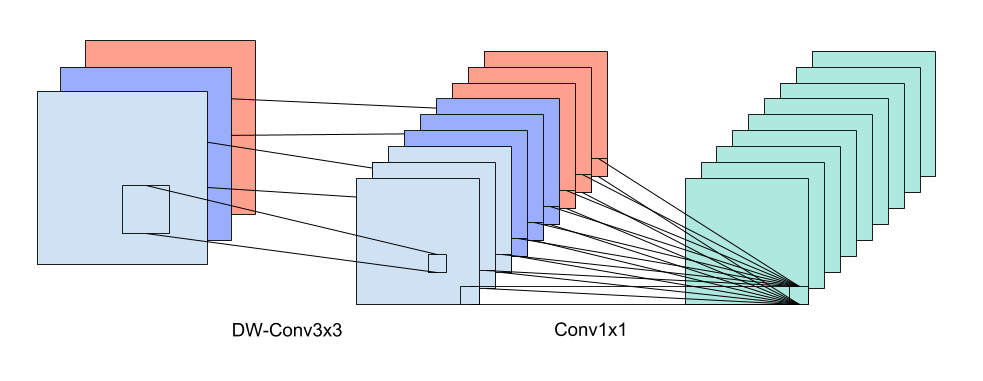
\includegraphics[width=\columnwidth]{figures/groupConvolutionPlusFusion.png}%
\caption{Convolution $3*3$ DeepWise suivie d'une convolution $1*1$ qui fait office de fusion.}%
\label{fig:conv31}%
\end{figure}

Au niveau de la complexité, une convolution $3*3$ sur 32 canaux d'entrée, avec 32 canaux de sortie, contient $ (3*3)*32*32 + 32 = 9248$ paramètres.
Une convolution $3*3$ DeepWise contient pour sa part uniquement $ (3*3)*32 + 32 = 320$ paramètres, comme on supprime toutes les connexions entre les canaux, soit 32 fois moins de connexion.
La convolution $1*1$ toujours avec 32 canaux contient $(1*1)*32*32 + 32 = 1056$ paramètres.
On obtient donc au final en combinant les deux $ 320 + 1056 = 1376$ paramètres, ce qui représente une diminution de 85\% par rapport au 9248 de la convolution $3*3$.


Nous comparons dans le tableau~\ref{tab:convG} les temps de calcul des différentes couches sur un processeur Quad Core cadencé à 2.60GHz, sous Linux 64 bits\footnote{Tous les calculs présentés dans la suite sont réalisés sur la même machine}, en utilisant le framework Pytorch\footnote{\url{https://pytorch.org}}. 
On observe une diminution passant de 23.9 millisecondes pour la convolution $3*3$ à 13.1 millisecondes pour la combinaison de la convolution $3*3$ DeepWise et de la convolution $1*1$, soit une diminution de 45\%. 
Nous utilisons les temps sur CPU, et non pas sur GPU, car nous nous intéressons au déploiement de notre réseau, et non pas à son entrainement, qui lui est réalisé sur GPU.
Pour obtenir des écarts stables et significatifs entre les différents runs, nous utilisons des batchs de 64 images, chacune d'une taille de $32*32$.

\begin{table}[!htb]
\centering
\begin{tabular}{|l|c|c|}
\hline
couche & \# paramètres & temps de calcul (ms) \\
\hline
\hline
Conv3x3 & 9248 & 23.9 \\
\hline
Conv3x3G & 320 & 9.94\\
\hline
Conv1x1 & 1056 & 4.06\\
\hline
Conv3x3G + Conv1x1 & 1376 & 13.1~\footnote{A noter que le temps de calcul de la convolution $3*3$ groupée suivie de la convolution $1*1$ n'est pas égal à la somme arithmétique des temps de calcul de chacune de ces opérations prises séparément. Cela vient de l'optimisation faite par le Framework utilisé (Ici Pytorch) dans l'enchaînement des opérations.} \\
\hline
\end{tabular}
\caption{Tableau de comparaison du nombres de paramètres et du temps de calculs des convolutions groupées et non groupées}
\label{tab:convG}
\end{table}

Nous avons donc un moyen de remplacer les convolutions $3*3$ pour minimiser le nombre de paramètres, et donc l'occupation mémoire, et les temps de calculs.
Cependant, nous souhaitons également tirer avantages des \textit{skip-connection} et de la régularisation.
Nous présentons dans la suite deux nouveaux types de blocs, remplaçant les convolutions $3*3$ par ce que nous avons présenté, et ajoutant des connexions et de la régularisation.


\subsection{Bloc S1}
\label{sec:S1}


Nous avons énoncé précédemment (section~\ref{sec:cnn}) l'utilité d'avoir deux types de blocs de convolutions, avec l’un qui conserve la taille des entrées que nous nommons S1, et l’autre qui divise par deux la taille des entrées, en multipliant le nombre de canaux, nommé S2.
Le bloc S1 que nous proposons est composé de la combinaison des convolutions présentées précédemment.
Tout d'abord une convolution $3*3$ DeepWise, avec un pas de 1 et un remplissage (padding) de 1, pour conserver la taille des entrées.
Ensuite, une convolution $1*1$ avec pas de 1 et pas de remplissage, chargée de faire la fusion des informations des différents canaux.
Pour améliorer la généralisation de notre réseau, nous ajoutons après chacune de ces couches, une \textit{batch-normalisation}.
Nous utilisons également le fait d'avoir remplacé la convolution $3*3$ par deux convolutions pour mettre une couche de neurones ReLU entre les deux, ce qui augmente la non-linéarité du bloc. 
Nous proposons également une \textit{skip-connection} entre l'entrée et la sortie du bloc, pour permettre une meilleur propagation du gradient~\cite{he2015delving}.
La figure~\ref{fig:S1} montre une représentation graphique du bloc S1, et le code qui réalise cette fonction est indiqué en annexe~\ref{sec:implementationS1}.


\begin{table}[!htb]
\centering
\begin{tabular}{|c|c|}
\hline
\#couche & type de couche \\
\hline
\hline
1 & convolution $3*3$ DeepWise, pas de 1, remplissage de 1 \\
\hline
2 & \textit{batch-normalisation}\\
\hline
3 & neurones ReLU\\
\hline
4 & convolution $1*1$, pas de 1, pas de remplissage\\
\hline
5 & \textit{batch-normalisation}\\
\hline
6 & neurones ReLU \\
\hline
7 & fusion des informations entre l'entrée et la sortie par addition\\
\hline

\end{tabular}
\caption{Composition du bloc S1.}
\label{tab:S1}
\end{table}



\begin{figure}%
\centering
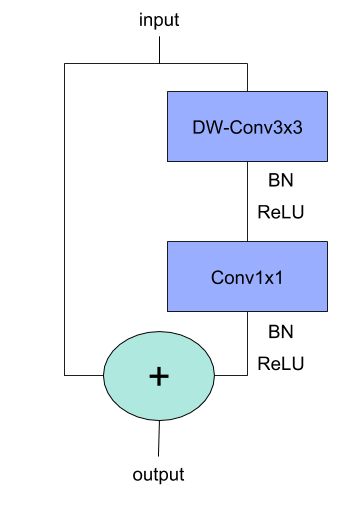
\includegraphics[width=.45\columnwidth]{figures/stride1.png}%
\caption{Schéma du module S1.}%
\label{fig:S1}%
\end{figure}

Les temps de calculs, rapportés dans le tableau~\ref{tab:blocS1}, montrent une large augmentation du temps de calcul, due à l'ajout de la \textit{batch-normalisation} et des couches ReLU.
Si on compare au tableau précédent, on passe de 13.1ms à 23.9ms.
Cependant, au niveau des paramètres, on ajoute ici uniquement ceux de la \textit{batch-normalisation}, ce qui donne un total 1504. 
Nous comparons notre bloc aux blocs ``Fires'' de SqueezeNet~\cite{iandola2016squeezenet} et ``Shuffle'' proposé par ShuffleNet~\cite{zhang2017shufflenet} dans le tableau~\ref{tab:blocS1}.
Ces deux blocs se basent sur la diminution du nombre de canaux entre les deux couches de convolutions, pour réduire le nombre de canaux d'entrée pour la convolution $3*3$, ce qui permet de réduire le nombre de paramètres.
Les deux réseaux doivent utiliser une coûteuse convolution $3*3$ en première couche pour extraires les premières informations de l'image.
Comme le bloc S1 a pour but de pouvoir remplacer toutes les convolutions, nous pouvons nous passer de cette couche, ce qui réduit le nombre de paramètres du réseau final.
On voit dans la tableau que le bloc S1 est plus lent, 23.9ms, que les bloc Fire (22.3ms) et Shuffle (21.8ms).
 

\begin{table}[h]
\centering
\begin{tabular}{|l|c|c|}
\hline
Bloc & \# paramètres & temps de calcul (ms) \\
\hline
\hline
Conv3x3DW + Conv1x1 & 1376 & 13.1 \\
\hline
Fire Bloc & 2888 & 22.3 \\
\hline
Shuffle Bloc & 472 & 21.8 \\
\hline
Bloc S1 & \textbf{1504} & \textbf{23.9}\\
\hline
\end{tabular}
\caption{Tableau de comparaison des blocs des réseaux de tailles réduites avec le bloc S1}
\label{tab:blocS1}
\end{table}

Notre bloc S1 permet donc de remplacer une convolution $3*3$, avec un nombre de paramètres inférieur et en ajoutant une \textit{skip-connection}.
Il est fait pour conserver la taille des tailles des entrées, en ne modifiants ni les tailles des filtres, ni le nombre de canaux.
Nous définissons dans la partie suivante le bloc S2, qui peut agir sur le nombre de canaux, et qui va diviser par deux la tailles des filtres d'entrée.


\subsection{Bloc S2}
\label{sec:S2}

Pour remplacer les convolutions qui réduisent la taille des entrées, et notamment la première couche $3*3$ utilisée par la plupart des résaux, nous définissons le bloc S2
Nous voulons toujours prendre avantage des \textit{skip-connection}, mais cette fois-ci nous avons une diminution de la taille de l'entrée et un changement du nombre de canaux, il n'est donc pas possible de directement additionner l'entrée et la sortie.
Tout d'abord le nombre de canaux étant différent, nous proposons de remplacer l'addition par une concaténation.
Ceci permet de garder les apports des \textit{skip-connection}, avec des résultats proches de ceux de l'addition~\cite{he2015delving, zhang2017shufflenet, ma2018shufflenet}.
Cependant, pour pouvoir réaliser la concaténation, chaque canal doit avoir la même taille.
Nous proposons donc de fixer le changement de taille à une division par deux de la taille.
Ainsi, inspiré par~\cite{ma2018shufflenet}, en appliquant un \textit{Average-Pooling} de $3*3$, avec un pas de 2 et un remplissage de 1, on obtient une sortie deux fois plus petite, qu'il est possible de concaténer à la sortie des couches de convolutions.

La partie convolution de ce bloc est très proche de celle du bloc S1, avec uniquement un changement de la première couche.
La couche de convolution $3*3$ DeepWise est appliquée avec un décalage de 2 et un remplissage de 2, ce qui a pour effet de diminuer la taille des entrées par deux.
Le nombre de canal de sortie du bloc est défini comme le double du nombre de canal d'entrée.
La bloc S2 (figure~\ref{fig:S2} représente la bloc S2, avec sur la partie gauche l'opération de Pooling pour diminuer la taille des entrées, et sur la droite, les couches de convolutions.

\begin{figure}%
\centering
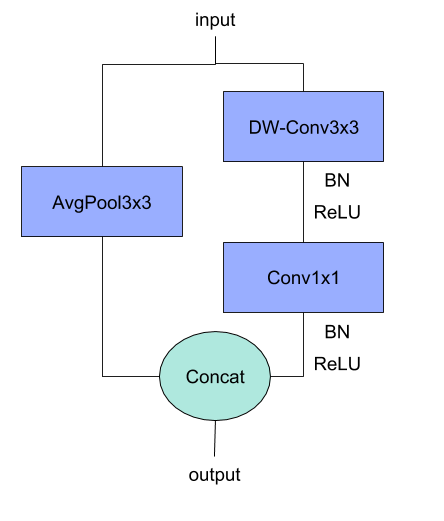
\includegraphics[width=.6\columnwidth]{figures/stride2.png}%
\caption{Schéma du module S2.}%
\label{fig:S2}%
\end{figure}


Le nombre de paramètres, observé dans la deuxième colonne du tableau~\ref{tab:blocS2}, ne change pas par rapport au bloc S1.
Nous pouvons le comparer au bloc Shuffle avec décalage de 2, qui utilise la concaténation aussi pour faire la fusion entre entrées et sorties.
Ce bloc à 848 paramètres, mais un temps d'exécution de 14.9ms, comparé à 13.2ms pour le bloc S2. 
Le bloc S2 est beaucoup plus rapide que le bloc S1, venant du fait qu'il applique deux fois moins les convolutions $3*3$, étant donné qu'il utilise un décalage de 1.

\begin{table}[h]
\centering
\begin{tabular}{|l|c|c|}
\hline
Bloc & \# paramètres & temps de calcul (ms) \\
\hline
\hline
Shuffle Bloc Stride 2 & 848 & 14.9 \\
\hline
Bloc S2 & \textbf{1504} & \textbf{13.2}\\
\hline
\end{tabular}
\caption{Tableau de comparaison des blocs ``Shuffle Stide 2'' et S2}
\label{tab:blocS2}
\end{table}



\subsection{Réseau de classification de gestes à base de S1 et S2}

Dans cette partie, nous construisons un réseau profond en utilisant les blocs S1 et S2.
Avec pour objectif d’obtenir un réseau avec un nombre de paramètres faible, et une vitesse d'exécution réduite par rapport aux réseau profonds de grandes taille, comme AlexNet ou ResNet, mais également plus petit que SqueezeNet ou ShuffleNet.
Inspiré par les micro-architectures récentes~\cite{howard2017mobilenets, zhang2017shufflenet,hu2017squeeze, iandola2016squeezenet} et également par VGG~\cite{simonyan2014very}, nous proposons de remplacer toutes les convolutions $3*3$ par des blocs S1, et toutes les convolution $3*3$ avec décalage de 2, qui font donc du sous échantillonnage, par le bloc S2. 

Comme montré sur la figure~\ref{fig:reseau1frame}, en partant d'une image $224*224*3$, on applique successivement les blocs S1 (sans réduire la taille) et S2 (en réduisant et en augmentant le nombre de canaux, jusqu'à obtenir une dimension suffisante pour la classification, ici $7*7*1024$.
Un \textit{Average-Pooling} de $7*7$ est alors appliqué, pour obtenir une matrice de $1*1*1024$.
Une couche entièrement connectée est alors utilisé pour réduire la dimension de 1024 à 6, notre nombre de gestes à reconnaître.

\begin{figure}
\centering
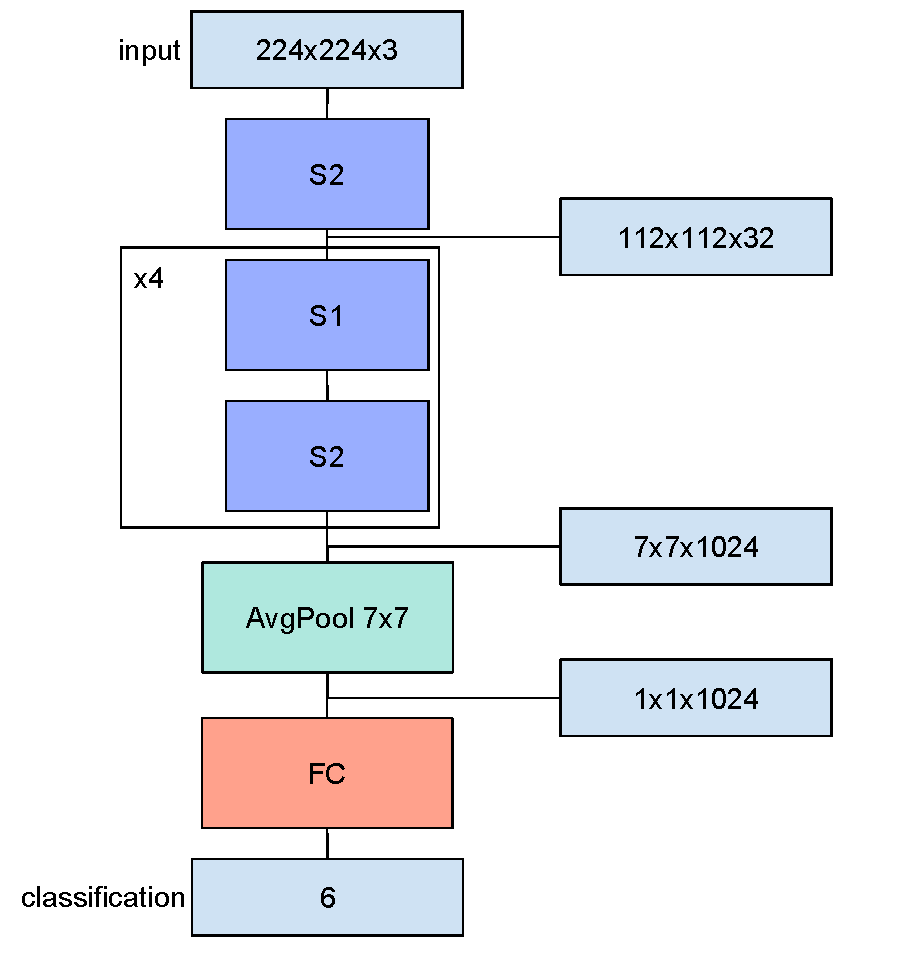
\includegraphics[width=\columnwidth]{figures/Reseau1frame.pdf}%
\caption{Schéma du réseau proposé pour la reconnaissance de geste, avec entre chaque connection la taille de la matrice de représentation des données.}%
\label{fig:reseau1frame}%
\end{figure}


Nous comparons notre réseau en terme de taille à des réseaux de petites tailles, tels que SqueezeNet, MobileNet et ShuffleNet, ainsi qu’à des réseaux comme AlexNet et ResNet pour donner une idée des ordres de grandeur.
Les résultats de cette comparaison sont présentés dans le tableau~\ref{tab:networkscomparison}.
Pour comparer ces réseaux entre eux, nous nous basons sur le même framework, c'est pourquoi les résultats peuvent différer de ceux présentés dans les publications originales respectives.
Les expérimentations sont réalisées avec des batch de 8 images de taille 224x224 à trois canaux.

Nous voyons que notre modèle est celui qui propose le moins de paramètres avec 772 millions de paramètres contre 922 millions, sans être pour autant le plus rapide 0.284 secondes contre 0.226 pour ShuffleNet.
Cela venant du fait que nous utilisons plus d'\textit{average-pooling} et de \textit{batch-normalisation} que les autres modèles.
L'objectif de notre réseau est de fournir une occupation mémoire la plus faible possible, pour pouvoir être utilisé sur mobile, à côté de notre réseau de reconnaissance d'instance (section~\ref{chap:regions}).
En terme de temps de calcul, il est de l'ordre de grandeur des réseau spécialisés pour les applications mobiles que sont MobileNet, SqueezeNet et ShuffleNet.

Nous n'avons donc pas de problème niveau temps d'exécution, et préférons optimiser l'utilisation de la mémoire, qui est dans notre cas plus problématique, dans le sens où elle doit être partagée avec le réseau de reconnaissance d'œuvres.

\begin{table}
\centering
\begin{tabular}{|l|c|c|}
\hline
\hline
Modèle & \# paramètres (en millions) & Temps de calcul (secondes) \\
\hline
SqueezeNet & 1.235 & 0.268 \\
\hline
MobileNet & 4.231 & 0.631~\footnote{Bien qu'ayant le nombre de paramètres et les mêmes couches que dans leur papier~\cite{howard2017mobilenets}, nous obtenons un réseau particulièrement lent, avec un réseau qui est normalement presque 40\% plus rapide que AlexNet. Nous mettons cela sur le compte de notre implémentation.} \\
\hline
ShuffleNet & 0.922 & \textbf{0.226} \\
\hline
Notre modèle & \textbf{0.772} & 0.284 \\
\hline
\hline
AlexNet & 61.100 & 0.380 \\
\hline
ResNet & 60.192 & 4.69 \\
\hline
\end{tabular}
\caption{Comparaison des réseaux de neurones, de petite et de grande taille.}
\label{tab:networkscomparison}
\end{table}

Notre réseau, qui nous nommons par la suite le modèle SimpleTrame, est un réseau de petite taille, adapté au processeur mobile, avec un temps d'exécution proche des micro-architecture de l'état de l'art.
Dans la partie suivante, nous nous intéressons aux performances de notre architecture dans la tâche de reconnaissance de geste dans les vidéos à la première personne.

\subsection{Evaluation}

Nous comparons notre réseau SimpleTrame avec les différentes réseaux de l'état de l'art présenté précédemment, sur la tâche de reconnaissance de geste.
Le corpus utilisé est présenté en annexe~\ref{sec:corpusGestes}. 
Il s'agit d'une collection de vidéo à la première personne, contenant les 6 gestes du projet GUIMUTEIC (5 geste + absence de geste).
Il est composé de 29 heures de vidéos, représentant 1669 séquences avec un geste et 1830 séquences sans gestes, ce qui fait un total de 120 000 images.
Ce corpus est séparé en trois groupes, 80\% de séquences d'entraînement, 10\% de séquence de validation et 10\% pour le test.
Les résultats rapportés dans le tableau~\ref{tab:singleframe} représentent la précision sur la partie test de cette collection.
Pour que la classification d'une séquence soit correcte, il faut que la majorité des images de la séquence soient classifiées correctement par le réseau.

\begin{table}
\centering
\begin{tabular}{|l|c|c|}
\hline
Modèle & \#paramètres (en million) & Précision (en pourcent) \\
\hline
\hline
SqueezeNet & 1.235 & 62.50  \\
\hline
MobileNet & 4.231 & 56.25  \\
\hline
ShuffleNet & 0.922 & 68.75  \\
\hline
SimpleTrame & \textbf{0.772} & 56.25  \\
\hline
AlexNet & 61.100 & 65.62 \\
\hline
ResNet & 60.192 & \textbf{71.87} \\
\hline
\end{tabular}
\caption{Comparaison de performance sur trame unique des différents réseaux.}
\label{tab:singleframe}
\end{table}

Notre réseau a une précision de 56.25\% sur le corpus geste GUIMUTEIC. 
Ce qui est similaire au résultats de MobileNet, avec moins de paramètres, 0.772 millions contre 4.231.
Les réseaux AlexNet, ShuffleNet et ResNet obtiennent de meilleurs résultats, avec un nombre de paramètres également supérieur.
Nos résultats sont ici inférieur à l'état de l'art, et ne permettent pas en l'état l'utilisation du réseau dans le cadre du projet GUIMUTEIC.
Cependant, ces résultats ne s'intéressent qu'à une seule trame de la vidéo pour la reconnaissance.
Dans la section suivante, nous proposons une version sur plusieurs trames de notre réseau, avec une fusion des informations venant de plusieurs instants de la video.



%%%%%%%%%%%%%%%%%%%%%%%%%%%%%%%%%%%%%%%%%%%%%%%%%%%%%%%%%%%%%%%%%%%%%%%%%%%%%%%%%%%%%%%%%%%%%%%%%%%%
%
%			Multi-Frame
%
%
%%%%%%%%%%%%%%%%%%%%%%%%%%%%%%%%%%%%%%%%%%%%%%%%%%%%%%%%%%%%%%%%%%%%%%%%%%%%%%%%%%%%%%%%%%%%%%%%%%%%
\section{Fusion d'information de plusieurs trames de la vidéo}
\label{sec:multiframe}

Les gestes à reconnaitre peuvent être dynamiques dans la vidéo, et pour identifier correctement la séquence, nous souhaitons tirer profit de l'information provenant de plusieurs trames de la vidéo.
Dans la section précédente, nous avons appliqué les réseaux de neurones sur chaque trame des vidéo, en classifiant chacune de ces images.
Il est cependant possible qu'un réseau considère plusieurs images.
Nous avons présenté dans la section~\ref{sec:stateVideo} les réseau récursifs.
Dans le cas des vidéos, les réseaux récursifs, utilisant les LSTM ou les GRU, sont utilisés sur la sortie d'un réseau convolutif pour réaliser une fusion des informations temporelle.
Ils ont l'avantage de ne pas avoir de limite sur le nombre d'images qu'ils peuvent regarder, mais ils ne sont pas adaptés à l'utilisation sur mobile, comme ils requièrent que chaque image soit passée au travers d'un CNN, ce qui peut être coûteux.
En utilisant une fenêtre d'observation fixe, il est possible de définir un réseau convolutifs qui s'intéresse à plusieurs images de la vidéo, en réalisant une fusion des informations~\cite{karpathy2014large}.
Dans cette section, nous nous intéressons à étendre notre réseau pour qu'il capte les informations de plusieurs trames, toujours en limitant le nombre de paramètres.

Nous proposons des nouveaux blocs qui respectent les informations venant de différentes trames (section~\ref{sec:FWconv}).
Pour réaliser la fusion des informations de plusieurs trames, nous utilisons à une convolution $1*1$, et nous évaluons l'impact de l'emplacement de cette fusion, au niveau performance, mais également au niveau du nombre de paramètres (section~\ref{sec:fusion}).

\subsection{FrameWise Convolution}
\label{sec:FWconv}

Dans les sections précédentes, nous nous sommes intéressé uniquement à une image, l'entrée d'un réseau était alors une matrice de taille $H*L*C$, où $H$ et $L$ ($224$ et $224$ dans nos expérimentation) sont la hauteur et la largeur des trames, $C$ le nombre de canaux (3 pour RGB).
Nous nous intéressons maintenant à un ensemble de trames, donc un certain nombre d'images à la suite les unes des autres.
Nous pouvons voir une suite d'image comme une matrice de dimension supérieure $H*L*C*T$, où $T$ est nombre de trame, que l'on peut aussi voir comme une matrice de dimension 3: $H*L*(C*T)$, en concaténant les canaux de chacune des images.

Nos blocs S1 et S2 présentés précédemment utilisent les convolutions DeepWise, où chaque canal de sortie n'est connecté qu'à un seul canal d'entrée.
Comme chaque convolution ne s'intéresse qu'à un seul canal, en augmentant le nombre de canaux d'entrée d'un facteur $T$ et le nombre de canaux de sortie du même facteur $T$, la convolution DeepWise est toujours applicable, sans mélanger l'information venant de plusieurs trames. 
En effet, les $C$ premiers canaux correspondent à l'image 1, les canaux $] C; 2*C ]$ contiennent les informations venant de la deuxième trames, et ainsi de suite.

La fusion des informations entre les canaux est faite dans les blocs S1 et S2 par la convolution $1*1$.
Pour que celle-ci ne mélange pas les informations venant de plusieurs trames, nous proposons de la remplacer par une convolution $1*1$ que nous nommons \textbf{FrameWise}.
Cette couche doit réaliser la fusion des informations des canaux pour trames, mais pas les informations venant de différentes trames.
Pour cela, nous appliquons la convolution par groupe, avec un nombre de groupe égal à $T$ le nombre de trames.

\begin{figure}%
\centering
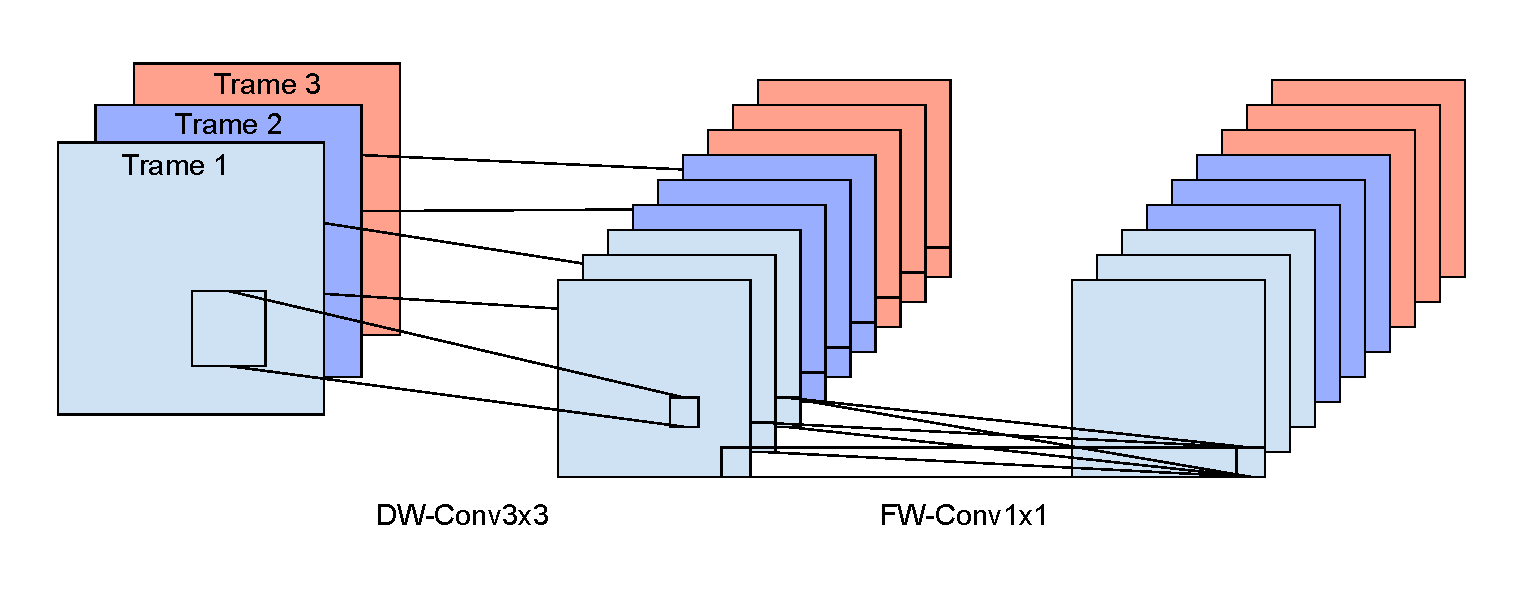
\includegraphics[width=\columnwidth]{figures/framewise2.pdf}%
\caption{Bloc de convolution utilisant DeepWise Convolution et FrameWise Convolution.}%
\label{fig:framewiseconv}%
\end{figure}

La figure~\ref{fig:framewiseconv}, montre une version modifiée de la figure~\ref{fig:conv31}, où les informations venant de chaque trames sont séparées.
En entrée, nous avons trois trames, chacune composé de 5 canaux.
La convolution $3*3$ DeepWise opère canal par canal, et le convolution FrameWise $1*1$ réalise une fusion des informations au niveau de chaque trame.

Cela nous permet de définir les nouveaux blocs nommés S1-FrameWise et S2-FrameWise, illustrés par le schéma~\ref{fig:framewiseS1S2}, en remplaçant uniquement la convolution $1*1$ par une convolution FrameWise.
Comme on augmente le nombre de convolutions réalisée, le nombre de paramètres va être multiplié par le nombre trames utilisés $T$.

\begin{figure}[!htb]
\centering
\begin{subfigure}{0.48\textwidth}
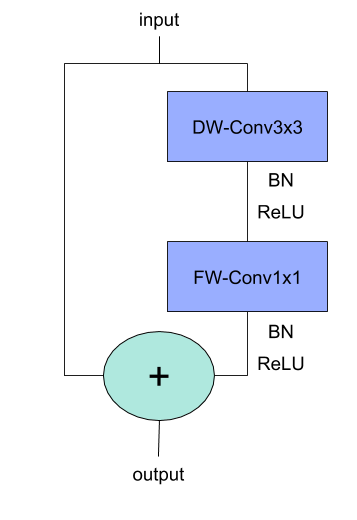
\includegraphics[width=\textwidth]{figures/stride1-FW.png}%
\caption{Bloc S1-FrameWise proposé.}%
\label{fig:FWS1}%
\end{subfigure}
\hspace*{\fill}
\begin{subfigure}{0.48\textwidth}
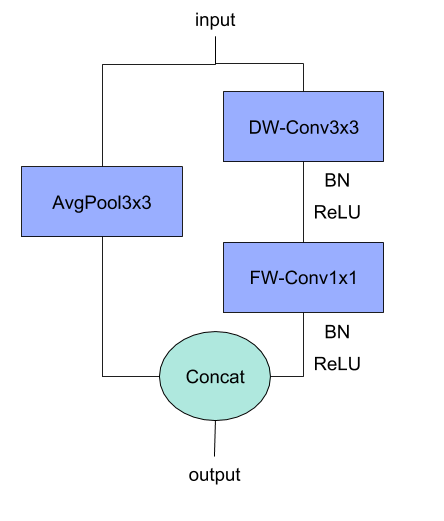
\includegraphics[width=\textwidth]{figures/stride2-FW.png}%
\caption{Bloc S2-FrameWise proposé.}%
\label{fig:FWS2}%

\end{subfigure}

\caption{Bloc S1 et S2 FrameWise.}
\label{fig:framewiseS1S2}
\end{figure}



\subsection{Fusion d'information de plusieurs trames}
\label{sec:fusion}

Enfin, à un moment dans le réseau, il faut fusionner l'information venant de l'ensemble des trames.
Nous définissons donc une couche de fusion, qui sera réalisée par une convolution $1*1$, comme nous avons montré précédemment que ce type de convolution était particulièrement adapté pour fusionner l'information entre les canaux.
De plus, à travers plusieurs expérimentation, nous n'avons pas remarqué de différences de précision entre l'utilisation d'un convolution $1*1$ et d'une convolution $3*3$. 
Etant donné que la convolution $1*1$ utlise 9 fois moins de paramètres, elle est donc à privilégier.

Nous définissons notre réseau, MultiTrame, qui est très similaire au réseau SimpleTrame~\ref{fig:reseau1frame}, la seule différence étant l'utilisation de bloc FrameWise, et de la couche de fusion.
Sur la figure~\ref{fig:reseau1}, nous montrons une des représentations possible du réseau MultiTrame.
Dans cet exemple, la fusion est réalisée au milieu du réseau, couche nommé conv1x1. 
Avant la fusion, les blocs utilisés sont des blocs FrameWise, on remarque sur la droite du schéma que la taille des matrices est plus grande, avec l'ajout du facteur $T$, le nombre de trames utilisées.
Après la fusion, le réseau est similaire au réseau SimpleTrame, avec l'utilisation de bloc S1 et S2.

\begin{figure}%
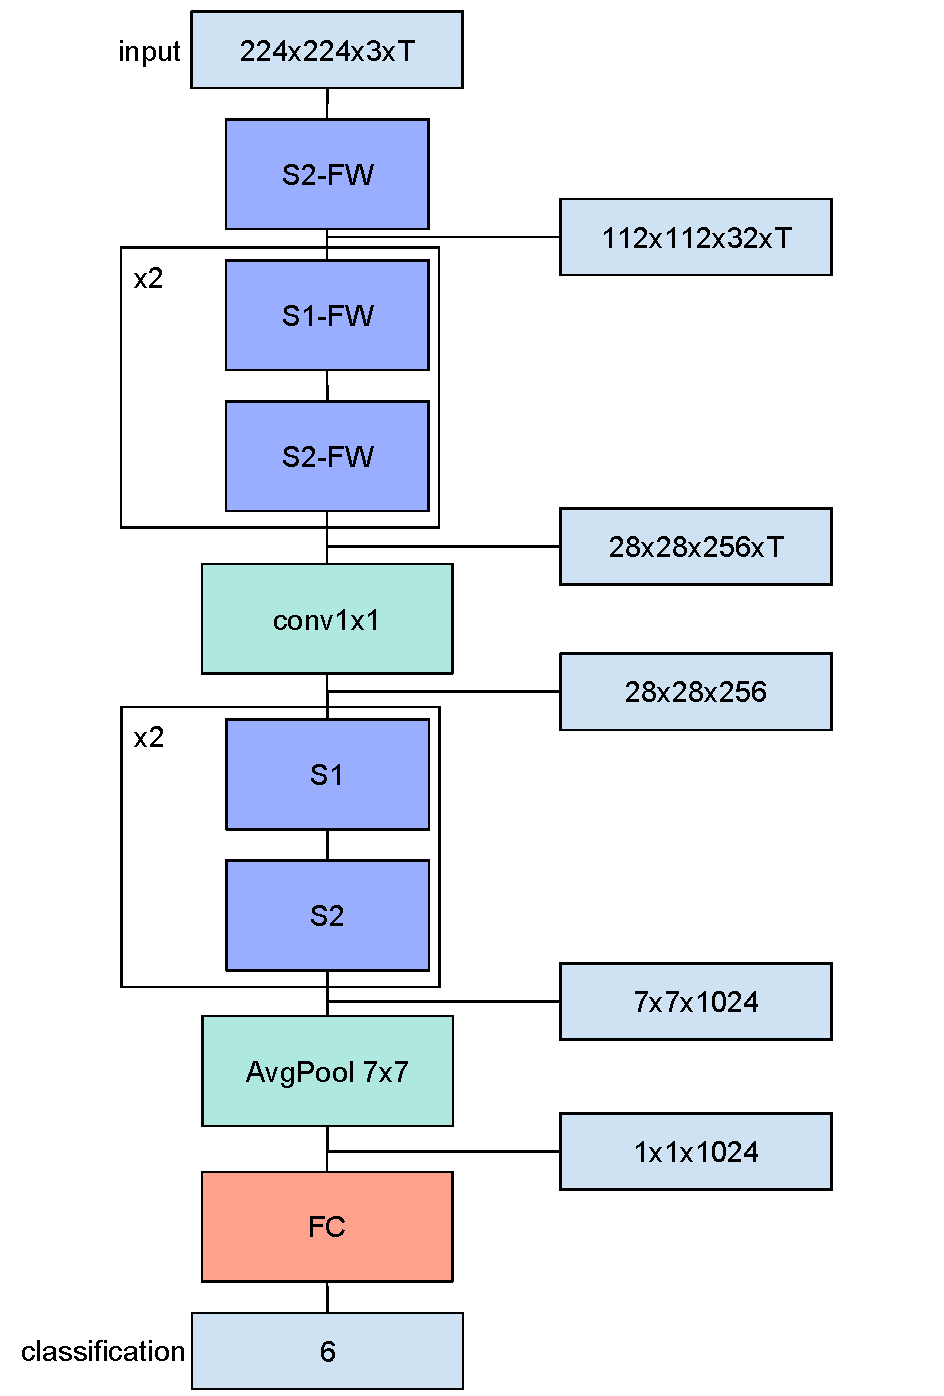
\includegraphics[width=.9\textwidth]{figures/Reseau1.pdf}%
\caption{Réseau proposé pour la détection de geste. Les premières couches sont sensibles à la trame (FrameWise), jusqu'à la fusion des $N$ trames par une convolution $1*1$.}%
\label{fig:reseau1}%
\end{figure}

La fusion peut être réalisée à plusieurs positions dans le réseau.
Dans l'exemple sur la figure~\ref{fig:reseau1}, elle est faite après le troisième bloc S2-FrameWise.
Cependant, il est possible la modifier le réseau pour que celle-ci soit réalisée plus profondément ou non dans le réseau.

Pour déterminer la position idéale de la fusion, en terme de performance et de nombre de paramètres, nous proposons de faire varier son emplacement dans le réseaux.
La modification de cette position entraîne un changement du nombre bloc FrameWise utilisé, et donc du nombre de paramètres.
Plus la fusion est réalisé tôt, plus on perd rapidement l’information temporelle, et plus le nombre de paramètre sera réduit.
En annexe~\ref{sec:multiframeSchemas}, nous présentons toutes les variantes utilisé pour le test.

Sur la courbe~\ref{fig:FusionLayer}, nous montrons l'impact de l'emplacement de la fusion sur la précision et sur la taille du réseau.
Les numéro 1 à 5 représente l’emplacement de la fusion, avec en 1, la première couche et en 5 la dernière couche.
En trait plein, avec la légende à gauche, nous notons la précision de la prédiction du réseau.
En trait pointillé, avec la légende à droite, nous reportons le nombre de paramètres.

Lorsque la fusion est réalisé sur la première couche, on retrouve la même précision qu'avec le réseau SimpleTrame. 
Dans ce cas, le réseau est en fait très similaire au réseau SimpleTrame, avec une fusion des informations temporelles réalisée dès le départ, tout le reste du réseau reste inchangé.
On remarque un pic de précision lorsque la fusion est réalisée au milieu de réseau, exemple montré dans la figure~\ref{fig:reseau1}.
En réalisant les fusion plus tardivement, on remarque une baisse des performances.
Cela est dû à un manque de généralisation du réseau, qui est dans un cas de sur-apprentissage.
Ceci pourrait être réglé par l'ajout de plus de régularisation ou en modifiant les hyper-paramètres de l'apprentissage, mais on remarque sur la courbe en pointillée la grande augmentation du nombre de paramètres.
Nous n’investiguons donc pas ce problème, car nous obtenons une performance optimale avec la fusion au milieu de réseau, et le nombre de paramètres restant proche du réseau simple, cette solution semble optimale.


\begin{figure}
\centering
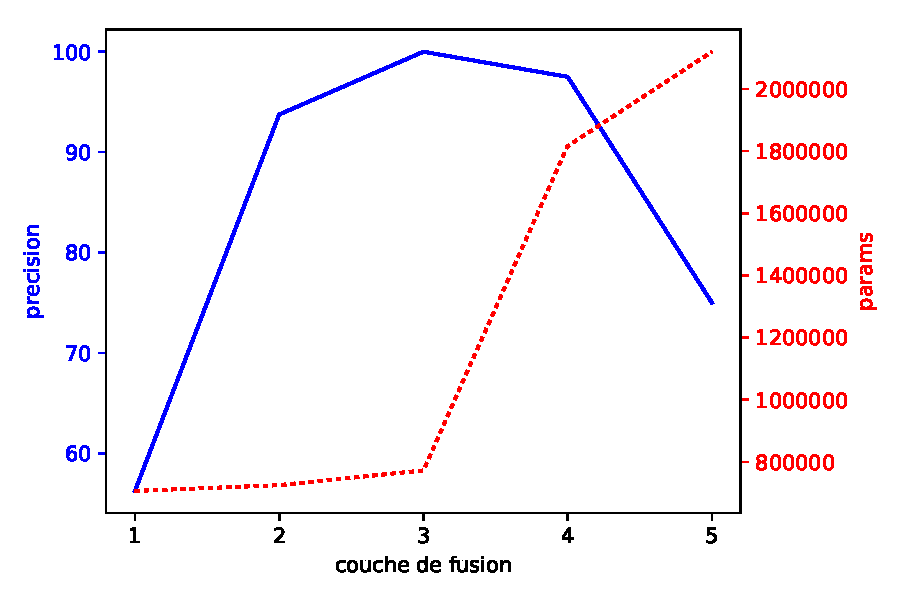
\includegraphics[width=\columnwidth]{figures/precisionFusion.pdf}
\caption{Courbe d'évaluation de la position de la fusion.}%
\label{fig:FusionLayer}%
\end{figure}

Dans le tableau~\ref{tab:fusion}, nous comparons notre réseau au réseau AlexNet et ShuffleNet, avec différentes méthodes de fusion.
La fusion 1 se réfère à la concaténation des canaux des différentes images sur la première couche du réseau, sans modifications du reste du réseau.
À l'exception d'une légère amélioration dans le cas d'AlexNet, ces résultats sont similaires à ceux obtenu sur trame unique.
La fusion EC, correspond à une fusion au niveau de la couche entièrement connectée du réseau, c'est-à-dire à la toute fin.
La réseau est dans ce cas plus grand, avec un nombre de paramètres multipliés par le nombre de trames, et n'obtient pas toujours les meilleurs résultats, notamment à cause de sur-apprentissage.
Pour AlexNet les résultats sont un peu différents, car c'est un réseau plus grand avec des hyper-paramètres bien connus pour éviter le sur-apprentissage. 
Nous le mettons ici dans le tableau pour montrer que les réseaux profonds classique obtiennent également 100\% de reconnaissance sur cette tâche.
La fusion au milieu du réseau comme présentée précédemment est la solution qui obtient les meilleurs résultats, avec un nombre de paramètres faible, ce qui correspond à notre objectif.
 

\begin{table}%
\centering
\begin{tabular}{|l|c|c|}

\hline
Modèle & Fusion & Score (en \%)\\
\hline
\hline
AlexNet & 1 & 68.75 \\
\hline
AlexNet & EC & 100.00\\
\hline
AlexNet & LSTM & 93.75\\
\hline
\hline
ShuffleNet & 1 & 68.75 \\
\hline
SqueezeNet & EC & 87.50 \\
\hline
\hline
Notre modèle & 1 & 56.25\\
\hline
Notre modèle & Milieu & 100.00\\
\hline
Notre modèle & EC & 75.00\\
\hline

\end{tabular}
\caption{Tableau de comparaison des différents modèles avec différentes fusion, plus ou moins hautes dans le réseau.}
\label{tab:fusion}
\end{table}


\section{Conclusion et limitations}

Nous avons présenté dans ce chapitre, un nouveau type de bloc pour la constructions de réseau de neurones profonds qui limitent grandement le nombre de paramètres, tout en permettant d'obtenir des résultats proches de ceux de l'état de l'art.
Les blocs S1 et S2 présentés utilise les convolution DeepWise, connus pour utiliser très peu de paramètres, et les \textit{skip-connection}, qui permettent une meilleur propagation du gradient, et un meilleur apprentissage.

Nous avons également proposé un nouveau type de blocs utilisant des convolutions FrameWise, qui respectent les informations venant de différentes trames de la vidéos.
Cela nous permet de définir un réseau qui réalise la fusion des informations des trames en son milieu, ce qui minimise l'augmentation du nombre de paramètres, en permettant d'obtenir les meilleurs résultats de reconnaissance de gestes.

Ces deux blocs, S1-FW et S2-FW, nous ont permis de définir un réseau de neurones utilisant très peu de paramètres, 20\% de moins que ShuffleNet.
Bien que n'obtenant pas d'aussi bon résultats que ce dernier, notre réseau à l'avantage d'être utilisable en mobilité plus facilement, grâce à une plus petite occupation mémoire.
Enfin, utilisé sur plusieurs trames, notre réseau obtient des performances à 100\% sur notre corpus de test, au même niveau que les réseaux des l'état de l'art, toujours avec un nombre de paramètres largement inférieur.
On en conclut que notre proposition permet bien d’être à l’état de l’art, tout en utilisant moins de paramètres, ce qui facilite son utilisation sur des outils mobiles.


